%!TEX TS-program = xelatex

% -- Document Class ------------------------------------------------------------

\documentclass[a4paper, 12pt]{article}

% -- Packages ------------------------------------------------------------------

% Language
\usepackage{polyglossia}
    \setmainlanguage{english}
    \setotherlanguage{german}
% Context sensitive quotation
\usepackage{csquotes}
% Citations
% \usepackage[style=alphabetic, backend=biber]{biblatex}
    % \addbibresource{References.bib}
% Extend options for positioning floats
\usepackage{float}
% Support highlighting of certain parts of the text
\usepackage{framed}
% Headers & Footers
\usepackage[automark, nouppercase]{scrpage2}
% To change the format of titles
\usepackage{titlesec}
% Support for unicode math fonts
\usepackage{unicode-math}
% Extended color support
\usepackage{xcolor}
% Extras for XƎTEX
\usepackage{xltxtra}
% Hyperlinks and pdf properties
\usepackage{hyperref}

% -- Macros --------------------------------------------------------------------

\newcommand{\Title}{Algorithmics}
\newcommand{\TitleDescription}{Exercises}
\newcommand{\Version}{1}
\newcommand{\Subject}
    {Solutions for the first exercise sheet of the course “Algorithmics”}
\newcommand{\KeyWords}{randomized algorithms, graph theory}
\newcommand{\LeftFooter}{Algorithmics}

\newcommand{\AuthorOne}{René Schwaiger}
\newcommand{\MailOne}{\href{mailto:sanssecours@f-m.fm}{sanssecours@f-m.fm}}

% Syntax highlighting definitions
\newcommand{\hlstd}[1]{\textcolor[rgb]{0,0,0}{#1}}
\newcommand{\hlnum}[1]{\textcolor[rgb]{0.69,0.49,0}{#1}}
\newcommand{\hlesc}[1]{\textcolor[rgb]{1,0,1}{#1}}
\newcommand{\hlstr}[1]{\textcolor[rgb]{0.75,0.01,0.01}{#1}}
\newcommand{\hlpps}[1]{\textcolor[rgb]{0.51,0.51,0}{#1}}
\newcommand{\hlslc}[1]{\textcolor[rgb]{0.51,0.51,0.51}{\it{#1}}}
\newcommand{\hlcom}[1]{\textcolor[rgb]{0.51,0.51,0.51}{\it{#1}}}
\newcommand{\hlppc}[1]{\textcolor[rgb]{0,0.51,0}{#1}}
\newcommand{\hlopt}[1]{\textcolor[rgb]{0,0,0}{#1}}
\newcommand{\hllin}[1]{\textcolor[rgb]{0.33,0.33,0.33}{#1}}
\newcommand{\hlkwa}[1]{\textcolor[rgb]{0,0,0}{\bf{#1}}}
\newcommand{\hlkwb}[1]{\textcolor[rgb]{0,0.34,0.68}{#1}}
\newcommand{\hlkwc}[1]{\textcolor[rgb]{0,0,0}{\bf{#1}}}
\newcommand{\hlkwd}[1]{\textcolor[rgb]{0,0,0.51}{#1}}

% -- Color Definitions ---------------------------------------------------------

% Background color for syntax highlighting
\definecolor{bgcolor}{rgb}      {1,     1,      1}

% Custom color definitions
\definecolor{aqua}{rgb}         {0,     0.56,   1}
\definecolor{bluegray}{rgb}     {0.22,  0.46,   0.84}
\definecolor{grape}{rgb}        {0.56,  0,      1}
\definecolor{orchid}{rgb}       {0.41,  0.13,   0.55}
\definecolor{orange}{rgb}       {1,     0.54,   0}
\definecolor{silver}{rgb}       {0.57,  0.57,   0.57}
\definecolor{turquoise}{rgb}    {0,     0.86,   0.84}

% -- Document Properties -------------------------------------------------------

% No indendation after paragraph
\setlength\parindent{0cm}

% Hyperref properties
\hypersetup
{
    pdftitle    = {\Title},
    pdfsubject  = {\Subject},
    pdfauthor   = {\AuthorOne},
    pdfkeywords = {\KeyWords},
    colorlinks  = true,
    linkcolor   = black,
    anchorcolor = black,
    citecolor   = silver,
    urlcolor    = orange
}

% -- Fonts ---------------------------------------------------------------------

% Use same size for numbers and other text
\defaultfontfeatures{Numbers=Lining}

% Set fonts for document
\setmainfont[Mapping=tex-text]{Avenir Next}
\setsansfont[Mapping=tex-text]{Ubuntu}
\setmonofont[Scale=MatchLowercase]{Menlo}
\setmathfont{Asana-Math.otf}

% Define font styles
\newfontfamily\Zapfino{Zapfino}

% -- Header And Footers --------------------------------------------------------

% Use normal font instead of italic font for head
\renewcommand{\headfont}{\normalfont}

% Set headers and footers
\ihead{\headmark}
\ohead{}
\ifoot{\LeftFooter}
\ofoot{\thepage}

% Set height of head
\setlength{\headheight}{1.8\baselineskip}

% Set thickness of separation line in header, footer
\setheadsepline{0.5pt}
\setfootsepline{0.5pt}

% -- Titlepage -----------------------------------------------------------------

\begin{document}

\begin{titlepage}

    \begin{center}
        % Title and title-description
        {\Huge\Zapfino \Title}
        \vskip 0.5cm
        {\Large\textit\TitleDescription}
        \vskip 1cm
        \hrule
        \vskip 0.5cm
        % Information about author
        \begin{tabular}{p{8cm}l}
            \AuthorOne  & \MailOne\\
        \end{tabular}
        \vskip 0.5cm
        \hrule
        \vskip 13.5cm
    \end{center}

    % Date and version number
    \begin{leftbar}
        \begin{tabular}{ll}
            \textbf{Version}    & \Version\\
            \textbf{Date}       & \today
        \end{tabular}
    \end{leftbar}

\end{titlepage}

% -- Table of Contents ---------------------------------------------------------

% Set section format for table of contents
\titleformat{\section}{\sffamily\bfseries}{}{0pt}{}[{\color{aqua}\hrule}]

% Set separation of dots between name of section and page number to such a high
% value that there will be no points in the table of contents
\makeatletter \renewcommand{\@dotsep}{10000} \makeatother
% Use blank header and footer
\pagestyle{empty}
% Start on new page
\newpage
% The table of contents starts at the second page
\setcounter{page}{2}
% Set table of contents
\tableofcontents

% -- Section & Paragraph Style -------------------------------------------------

% Set format for section
\titleformat{\section}
    {\large\sffamily\bfseries}  % Large, bold, sans serif font for section
    {}                          % No format applied to whole title
    {0pt}                       % No separation between label and title
    {\thesection~·~}            % Start with section number
    [{\color{aqua}\hrule}]      % Underline with blue ruler

% Set format for other sections and paragraphs
% Color = orchid, Font = bold, sans serif
\titleformat*{\subsection}{\color{orchid}\sffamily\bfseries}
\titleformat*{\subsubsection}{\color{orchid}\sffamily\bfseries}
\titleformat*{\paragraph}{\color{orchid}\sffamily\bfseries}
\titleformat*{\subparagraph}{\color{orchid}\sffamily\bfseries}

% -- Page Style ----------------------------------------------------------------

% Start with text on a new page
\newpage
% Display headers and footers
\pagestyle{scrheadings}

% -- Text ----------------------------------------------------------------------

\section{Exercise 7 (Planar Graphs)}

\begin{itemize}

    \item Show that $m ≤ 3n − 6$ holds for any simple planar graph with $n ≥ 3$
    vertices and m edges.

    \item Show that $m ≤ 2n − 4$ holds for any simple planar bipartite graph
    with $n ≥ 3$ vertices and m edges.

    \item Use Euler’s formula to show that each simple, planar graph contains a
    vertex $v$ of degree $d(v) ≤ 5$.

\end{itemize}

\section{Exercise 9 (Floyd-Warshal Algorithm)}

Apply the Floyd-Warshal algorithm as presented in the lecture to the given
graph.

\begin{center}
    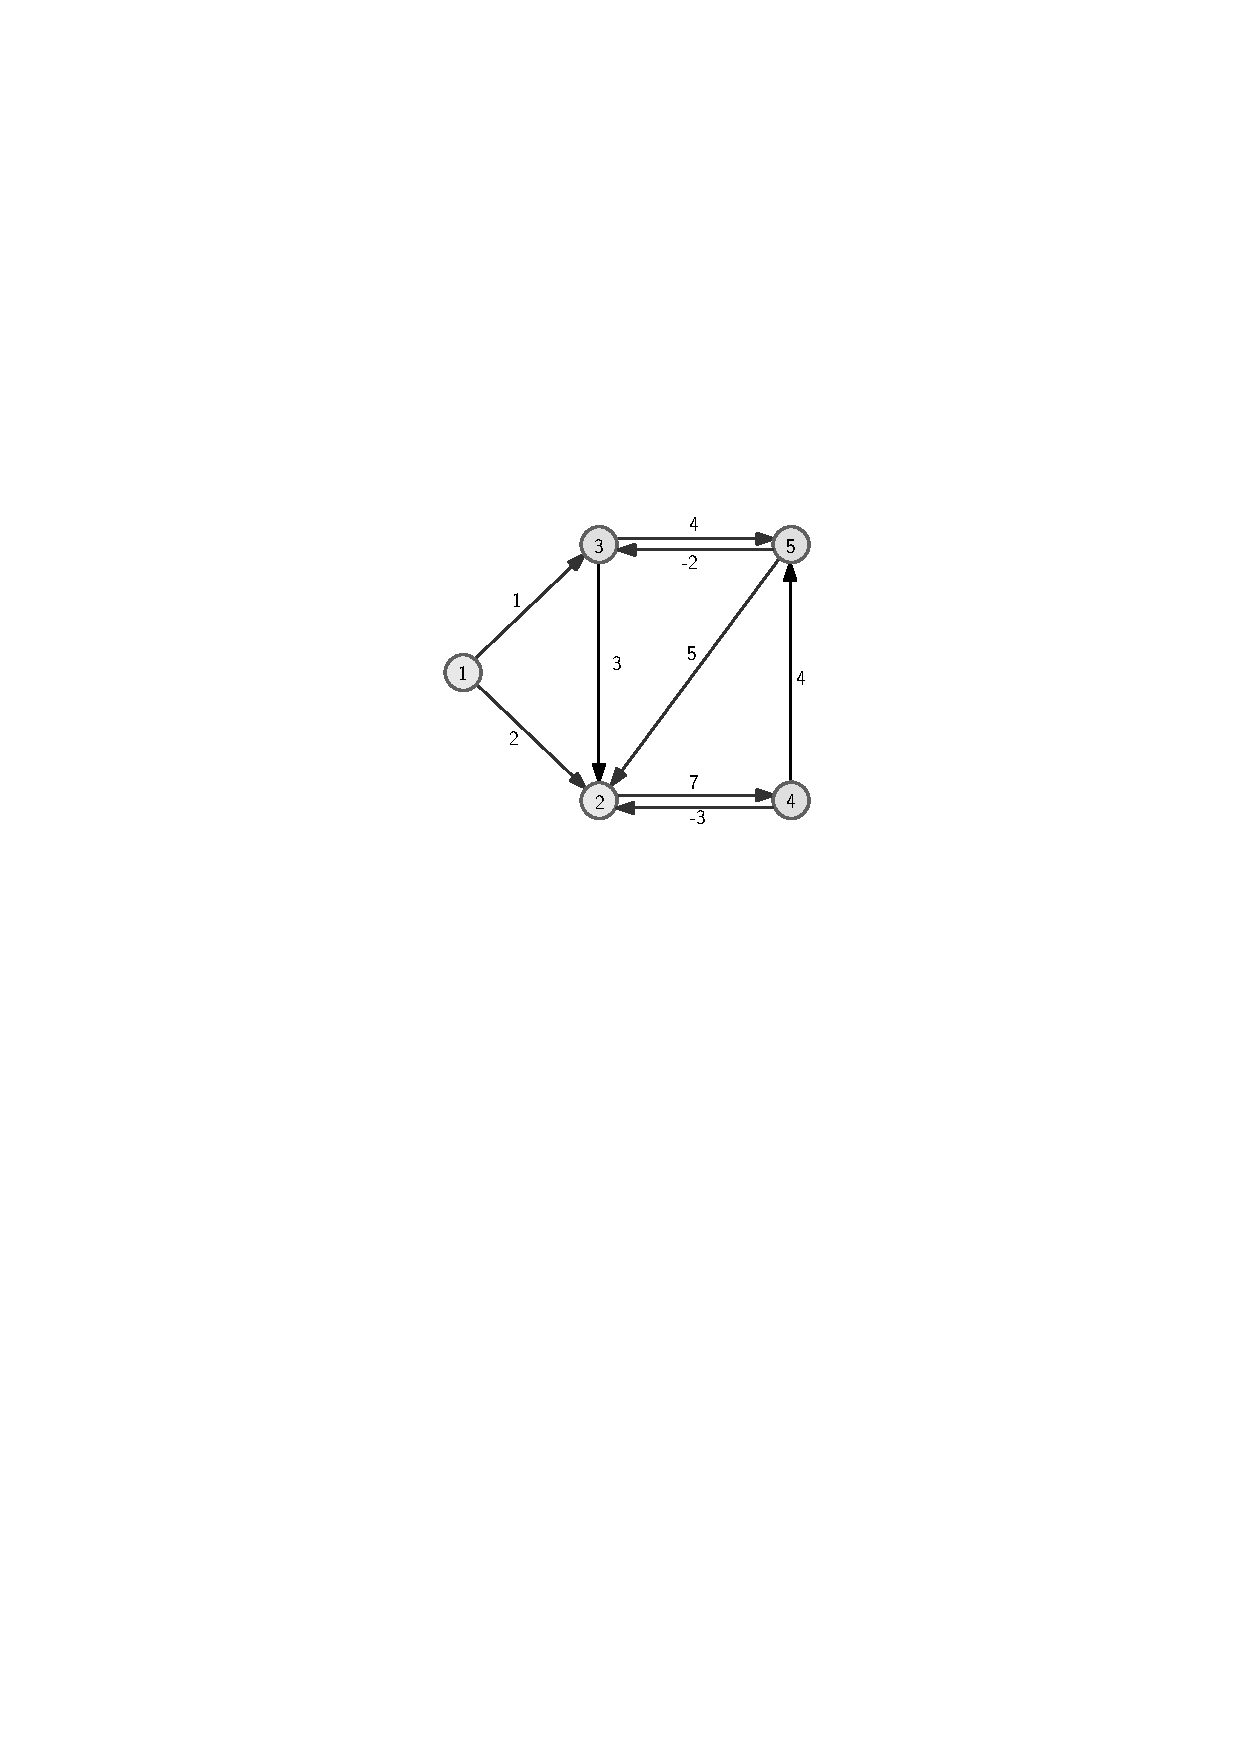
\includegraphics[width=0.5\textwidth]{Figures/Exercise_9}
\end{center}

\[
W = D^{(1)} =
\left(
    \begin{array}{ccccc}
        \textcolor{orange}{0}   &
        \textcolor{orange}{2}   &
        \textcolor{orange}{1}   &
        \textcolor{orange}{∞}   &
        \textcolor{orange}{∞}   \\

        \textcolor{orange}{∞}   &   0   &   ∞   &   7   &   ∞   \\
        \textcolor{orange}{∞}   &   3   &   0   &   ∞   &   4   \\
        \textcolor{orange}{∞}   &   -3  &   ∞   &   0   &   4   \\
        \textcolor{orange}{∞}   &   5   &   -2  &   ∞   &   0   \\
    \end{array}
\right)
\]

\begin{minipage}[b]{0.5\linewidth}
\[
D^{(2)} =
\left(
    \begin{array}{ccccc}
        0   &   \textcolor{orange}{2}   &   1   &   ∞   &   ∞   \\

        \textcolor{orange}{∞}   &
        \textcolor{orange}{0}   &
        \textcolor{orange}{∞}   &
        \textcolor{orange}{7}   &
        \textcolor{orange}{∞}   \\

        ∞   &   \textcolor{orange}{3}   &   0   &   ∞   &   4   \\
        ∞   &   \textcolor{orange}{-3}  &   ∞   &   0   &   4   \\
        ∞   &   \textcolor{orange}{5}   &   -2  &   ∞   &   0   \\
    \end{array}
\right)
\]
\end{minipage}
\begin{minipage}[b]{0.5\linewidth}
\[
D^{(3)} =
\left(
    \begin{array}{ccccc}
        0   &   2   &   \textcolor{orange}{1}   &   9   &   ∞   \\
        ∞   &   0   &   \textcolor{orange}{∞}   &   7   &   ∞   \\

        \textcolor{orange}{∞}   &
        \textcolor{orange}{3}   &
        \textcolor{orange}{0}   &
        \textcolor{orange}{10}  &
        \textcolor{orange}{4}   \\

        ∞   &   -3  &   \textcolor{orange}{∞}   &   0   &   4   \\
        ∞   &   5   &   \textcolor{orange}{-2}  &   12   &   0  \\
    \end{array}
\right)
\]
\end{minipage}

\begin{minipage}[b]{0.5\linewidth}
\[
D^{(4)} =
\left(
    \begin{array}{ccccc}
        0   &   2   &   1   &   \textcolor{orange}{9}   &   5   \\
        ∞   &   0   &   ∞   &   \textcolor{orange}{7}   &   ∞   \\
        ∞   &   3   &   0   &   \textcolor{orange}{10}  &   4   \\

        \textcolor{orange}{∞}   &
        \textcolor{orange}{-3}  &
        \textcolor{orange}{∞}   &
        \textcolor{orange}{0}   &
        \textcolor{orange}{4}   \\

        ∞   &   1   &   -2  &   \textcolor{orange}{8}   &   0   \\
    \end{array}
\right)
\]
\end{minipage}
\begin{minipage}[b]{0.5\linewidth}
\[
D^{(5)} =
\left(
    \begin{array}{ccccc}
        0   &   2   &   1   &   9   &   \textcolor{orange}{5}   \\
        ∞   &   0   &   ∞   &   7   &   \textcolor{orange}{11}  \\
        ∞   &   3   &   0   &   10  &   \textcolor{orange}{4}   \\
        ∞   &   -3  &   ∞   &   0   &   \textcolor{orange}{4}   \\

        \textcolor{orange}{∞}   &
        \textcolor{orange}{1}   &
        \textcolor{orange}{-2}  &
        \textcolor{orange}{8}   &
        \textcolor{orange}{0}   \\
    \end{array}
\right)
\]
\end{minipage}

\begin{minipage}[b]{0.5\linewidth}
\[
D^{(6)} =
\left(
    \begin{array}{ccccc}
        0   &   2   &   1   &   9   &   5   \\
        ∞   &   0   &   9   &   7   &   11  \\
        ∞   &   3   &   0   &   10  &   4   \\
        ∞   &   -3  &   2   &   0   &   4   \\
        ∞   &   1   &   -2  &   8   &   0   \\
    \end{array}
\right)
\]
\end{minipage}
\begin{minipage}[b]{0.5\linewidth}
\end{minipage}

\section{Exercise 10 (Johnson’s Algorithm)}

Calculate the values $hᵢ$ and $\hat{w}_{ij}$ as it is done by Johnson’s
algorithm for the graph of exercise 9.

\begin{minipage}[b]{0.5\linewidth}
\[
A' =
\left(
    \begin{array}{cccccc}
        0   &   0   &   0   &   0   &   0   &  0    \\
        ∞   &   0   &   2   &   1   &   ∞   &  ∞    \\
        ∞   &   ∞   &   0   &   ∞   &   7   &  ∞    \\
        ∞   &   ∞   &   3   &   0   &   ∞   &  ∞    \\
        ∞   &   ∞   &   -3  &   ∞   &   0   &  4    \\
        ∞   &   ∞   &   5   &   -2  &   ∞   &  0    \\
    \end{array}
\right)
\]
\end{minipage}
\begin{minipage}[b]{0.5\linewidth}
\begin{center}
    \begin{tabular}{c|cccccc}
        &  $δ_s$ &  $δ₁$  &  $δ₂$  &  $δ₃$  &  $δ₄$  &  $δ₅$\\
    \hline
    0   &  0     &  ∞      &  ∞      &  ∞      &  ∞      &  ∞    \\
    1   &  0     &  0      &  0      &  0      &  0      &  0    \\
    2   &  0     &  0      &  -3     &  -2     &  0      &  0    \\
    3   &  0     &  0      &  -3     &  -2     &  0      &  0    \\
    4   &  0     &  0      &  -3     &  -2     &  0      &  0    \\
    5   &  0     &  0      &  -3     &  -2     &  0      &  0    \\
    \hline
        &  $h_s$ &  $h₁$  &  $h₂$  &  $h₃$  &  $h₄$  &  $h₅$\\
    \end{tabular}
\end{center}
\end{minipage}

\begin{figure}[htbp]
    \caption{Graph for Johnson's Algorithm with initial weights}
    \vskip 0.2cm
    \centering
    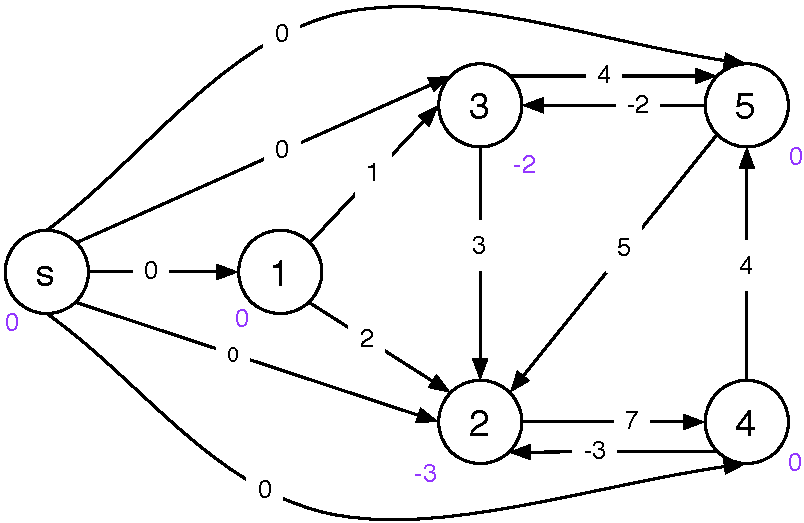
\includegraphics[width=0.6\textwidth]{Figures/Exercise_10_Initial}
    \label{figure:Exercise_10_Initial}
\end{figure}

\begin{figure}[htbp]
    \caption{
        Graph for Johnson's Algorithm with modified weight function
        $\hat{w}_{ij}$
    }
    \vskip 0.2cm
    \centering
    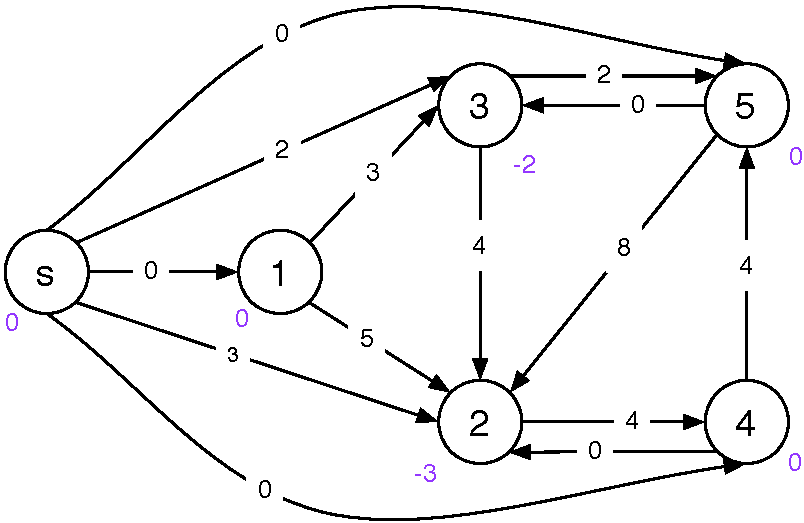
\includegraphics[width=0.6\textwidth]{Figures/Exercise_10_Modified_Weights}
    \label{figure:Exercise_10_Modified_Weights}
\end{figure}

\[
A =
\left(
    \begin{array}{cccccc}
       0   &   5   &   3   &   ∞   &  ∞    \\
       ∞   &   0   &   ∞   &   4   &  ∞    \\
       ∞   &   4   &   0   &   ∞   &  2    \\
       ∞   &   0   &   ∞   &   0   &  4    \\
       ∞   &   8   &   0   &   ∞   &  0    \\
    \end{array}
\right)
\]

% -- Bibliography --------------------------------------------------------------

% Set section format for bibliography
% \titleformat{\section}{\sffamily\bfseries}{}{0pt}{}[{\color{aqua}\hrule}]
% Display bibliography
% \printbibliography

\end{document}
